
\section{Εκτίμηση 3D ανθρώπινης πόζας}
\label{section:human_pose_estimation}

Η εκτίμηση της 3D ανθρώπινης πόζας είναι μία περίπλοκη διαδικασία, απαιτώντας έναν τρόπο λήψης των καρέ εισόδου από την κάμερα του χρήστη ή από ένα βίντεο εισόδου, την επεξεργασία των καρέ σε συγκεκριμένη μορφή, μία βιβλιοθήκη μηχανικής μάθησης και φυσικά το μοντέλο του βαθιού νευρωνικού δικτύου που διεξάγει τις εκτιμήσεις. Επομένως, στην συνέχεια του κεφαλαίου θα αναπτυχθούν ακριβώς αυτά τα εργαλεία που φέρουν σε πέρας τις αναφερθείσες διαδικασίες.

\subsection{NumPy}
\begin{figure}[h]
	\centering
	
\includegraphics[scale=0.4]{images/chapter3/numpy_logo.png}
	\caption{Λογότυπο της βιβλιοθήκης NumPy }
\end{figure}
Η βιβλιοθήκη Numerical Python (εν συντομία \textsl{NumPy})\footnote{\href{https://numpy.org/}{https://numpy.org/}} χρησιμοποιείται για την διαχείριση μεγάλων, πολλών διαστάσεων λιστών και πινάκων, προσφέροντας επίσης μία εκτενή συλλογή μαθηματικών συναρτήσεων υψηλού επιπέδου για την επεξεργασία αυτών. Η NumPy είναι βιβλιοθήκη ανοιχτού κώδικα και χρησιμοποιείται κατά κόρων από την επιστημονική κοινότητα με πληθώρα συνεισφορών.

Η NumPy χρησιμοποιεί την υλοποίηση αναφοράς CPython της Python, η οποία όμως όντας διερμηνέας δεν βελτιστοποιεί τον κώδικα. Τοιουτοτρόπως, αλγόριθμοι που τρέχουν πάνω σε αυτόν τείνουν να είναι πιο αργοί από αντίστοιχους που έχουν μεταγλωττιστεί. Η NumPy αντιμετωπίζει την αργή εκτέλεση παρέχοντας πολυδιάστατες δομές πινάκων και συναρτήσεων επεξεργασίας τους, οι οποίοι είναι αποδοτικοί. Προς επίτευξη αυτού του σκοπού, η NumPy:

\begin{itemize}
	\item Παρέχει πίνακες κοινών τύπων δεδομένων που στοιβάζονται πυκνά στην μνήμη. Οι λίστες της Python μπορούν να έχουν διαφορετικούς τύπους δεδομένων θέτοντας περιορισμούς καθώς διεξάγονται υπολογισμοί.
	\item Χωρίζει τις διεργασίες σε υποδιεργασίες και τις επεξεργάζεται παράλληλα.
	\item Χρησιμοποιεί εσωτερικά τη διεπαφή ξένων συναρτήσεων (Foreign Language Interface, \textsl{FFI}) της CPython, μέσω της οποίας επιτρέπεται η εκτέλεση ρουτινών και η χρήση υπηρεσιών διαφορετικής γλώσσας, όπως της C.
\end{itemize}


Η NumPy χρησιμοποιείται στην εκτίμηση πόζας εκτενώς τόσο για την αποθήκευση των διάφορων δεδομένων σε αποδοτικές δομές όσο και για την γρήγορη επεξεργασία τους. Μερικά παραδείγματα χρήσης της NumPy αποτελούν η αποθήκευση και επεξεργασία της έγχρωμης εικόνας καρέ σε έναν πίνακα διαστάσεων ΜxΝx3 (όπου Μ o αριθμός των πίξελ μήκους, Ν τα πίξελ πλάτους και τα 3 κανάλια χρώματος RGB\footnote{Στο πρότυπο χρώματος RGB ένα οποιοδήποτε χρώμα μπορεί να παραχθεί συνδυάζοντας προσθετικά τις τιμές από τα τρία βασικά χρώματα κόκκινου (\textbf{R}ed), πράσινου (\textbf{G}reen) και μπλε (\textbf{B}lue).}), καθώς και η αποθήκευση και επεξεργασία της εξόδου του νευρωνικού σε δύο πίνακες διαστάσεων 6980x3 (οι 3D συντεταγμένες των 6980 κορυφών πλέγματος) και 24x3 (οι συντεταγμένες των 24 σημείων κλειδιών).


\subsection{OpenCV}
\label{sec:opencv}
\begin{figure}[h]
	\centering
	
\includegraphics[scale=0.4]{images/chapter3/opencv_logo.png}
	\caption{Λογότυπο της βιβλιοθήκης OpenCV }
\end{figure}

Η Open Source Computer Library (εν συντομία \textsl{OpenCV})\footnote{\href{https://opencv.org/}{https://opencv.org/}} είναι μία βιβλιοθήκη προγραμματιστικών συναρτήσεων γραμμένων σε C++, παρέχοντας όμως APIs και σε άλλες γλώσσες όπως Python, Java και Matlab/Octave. Η OpenCV είναι μία διαπλατφορμική βιβλιοθήκη ανοιχτού κώδικα παρέχοντας πλήθος αλγορίθμων για υπολογιστική όραση και επεξεργασία εικόνας.

Η OpenCV χρησιμοποιείται στην εφαρμογή εκτίμησης πόζας κυρίως για την δυνατότητα λήψης εικόνων καρέ από κάποια πηγή. Συγκεκριμένα, η OpenCV παρέχει την κλάση \texttt{VideoCapture} η οποία όταν αρχικοποιείται δέχεται ως είσοδο την πηγή, η οποία μπορεί να είναι είτε η κάμερα του χρήστη είτε ένα αρχείο βίντεο. Έπειτα, καλώντας την συνάρτηση \texttt{read()} του αντικειμένου της κλάσης λαμβάνεται μία εικόνα καρέ από την πηγή, η οποία κατά την διαδικασία της αποσφαλμάτωσης προβάλλεται σε ειδικό παράθυρο με χρήση της συνάρτησης \texttt{imshow()} της OpenCV.

\subsection{Tensorflow}
\begin{figure}[h]
	\centering
	
\includegraphics[scale=0.7]{images/chapter3/tensorflow_logo.png}
	\caption{Λογότυπο της βιβλιοθήκης Tensorflow}
\end{figure}

To Tensorflow\footnote{\href{https://www.tensorflow.org/}{https://www.tensorflow.org/}} είναι μία πλατφόρμα από άκρη σε άκρη για μηχανική μάθηση. Αποτελείται από ένα ευρύ, ευέλικτο οικοσύστημα εργαλείων, βιβλιοθηκών και πόρους από την κοινότητα που επιτρέπει στους ερευνητές να εξελίξουν την τελευταία λέξη της τεχνολογίας στη μηχανική μάθηση και στους προγραμματιστές να αναπτύξουν και να ανεβάσουν με ευκολία εφαρμογές μηχανικής μάθησης.

Το Tensorflow εκτελεί πράξεις με τανυστές (\textsl{tensors}), οι οποίοι με απλά λόγια είναι πολυδιάστατοι πίνακες όπως φαίνεται στο Σχήμα \ref{fig:tensor_example}. H αλληλουχία των υπολογισμών στους τανυστές περιγράφεται από έναν στατικό κατευθυνόμενο άκυκλο γράφο (βλ. παράρτημα \ref{definition:directed_acyclic_graph}), ονομαζόμενου υπολογιστικός γράφος (computational graph), ο οποίος καθορίζεται πριν την εκτέλεση του μοντέλου. Η επικοινωνία του μοντέλου με την εφαρμογή επιτυγχάνεται μέσω των αντικειμένων \texttt{Session}, που επιτρέπει την εκτέλεση ενός γράφου ή τμήμα αυτού διανέμοντας τους πόρους του συστήματος και αποθηκεύοντας τιμές μεταβλητών και αποτελεσμάτων, και των αντικειμένων τύπου \texttt{Placeholder}, που είναι τανυστές οι οποίοι αντικαθίστανται από συγκεκριμένες τιμές κατά την εκτέλεση του μοντέλου. Για παράδειγμα ο παρακάτω κώδικας θα παρήγαγε τον υπολογιστικό γράφο που φαίνεται στο Σχήμα \ref{fig:computational_graph}.

\begin{minted}{python}
a = 15
b = 5
prod = a * b
sum = a + b
result = prod / sum
print(result)
\end{minted}

\begin{figure}[H]
	\centering
	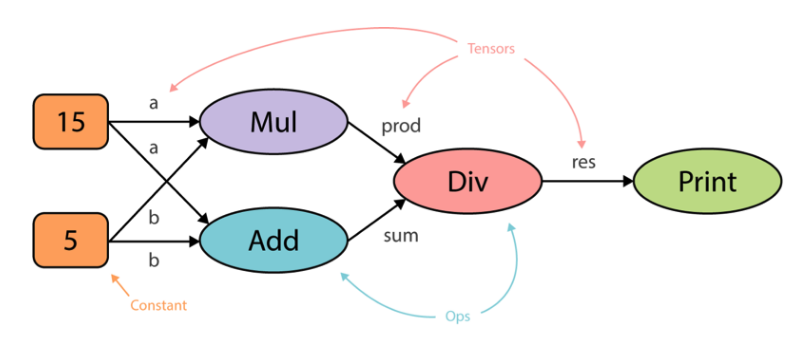
\includegraphics[scale=0.4]{images/chapter3/computation_graph.png}
	\caption[Παράδειγμα υπολογιστικού γράφου]{\textsl{Παράδειγμα υπολογιστικού γράφου}. Οι τανυστές $a$ και $b$ περνάνε από τους κόμβους υπολογισμού \texttt{Mul} και \texttt{Add} παράγοντας τους τανυστές \texttt{prod} και \texttt{sum} αντίστοιχα.}
	\label{fig:computational_graph}
\end{figure}

\begin{figure}[h]
	\centering
	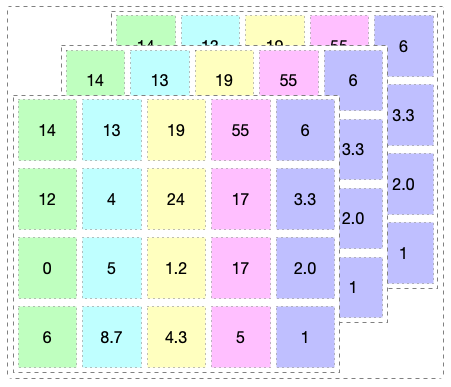
\includegraphics[scale=0.7]{images/chapter3/tensor_example.png}
	\caption{Παράδειγμα τανυστή}
	\label{fig:tensor_example}
\end{figure}

Με αυτό τον τρόπο, ο υπολογιστικός γράφος παράγεται με στατικό τρόπο πριν την εκτέλεση του κώδικα. Το κύριο πλεονέκτημα του στατικού γράφου είναι ότι επιτρέπει παραλληλισμό και χρονοπρογραμματισμό βασισμένο στις εξαρτήσεις των τανυστών καθιστώντας την εκπαίδευση του νευρωνικού δικτύου πιο γρήγορη και αποδοτική. Από την άλλη μεριά, ο στατικός γράφος θέτει περιορισμούς κατά την εκτέλεση του μοντέλου, απαιτώντας το μήκος της εισόδου να είναι σταθερό, το οποίο είναι αρκετά περιοριστικό σε ορισμένες περιπτώσεις που απαιτείται δυναμική μορφή εισόδου. Για παράδειγμα, σε ένα μοντέλο ανάλυσης συναισθήματος από κείμενο θα έπρεπε να ορισθεί σταθερό μήκος προτάσεων (γεμίζοντας τις μικρότερες προτάσεις με μηδενικά) μειώνοντας ενδεχομένως την απόδοση του μοντέλου.

Ένα άλλο χαρακτηριστικό του Tensorflow, που αποδεικνύει την ωριμότητα του ως πλατφόρμα, αποτελεί το πλαίσιο λογισμικού TensorFlow Serving. Αυτό είναι ένα ευέλικτο, υψηλής απόδοσης σύστημα σερβιρίσματος μοντέλων μηχανικής μάθησης. Το TensorFlow Serving επιτρέπει το εύκολο και γρήγορο στήσιμο ενός HTTP ή gRPC server όπου ανεβάζεται το εκπαιδευμένο μοντέλο. Στην συνέχεια, παρέχεται ένα RESTful API με το οποίο γίνεται δυνατή η χρήση του μοντέλου για εξαγωγή προβλέψεων. Τοιουτοτρόπως, σε αντίστοιχες εφαρμογές με περιορισμένους υπολογιστικούς πόρους μπορεί να αποδεσμευτεί το μοντέλο μηχανικής μάθησης από την υπόλοιπη εφαρμογή, επιτρέποντας την εκτέλεση αλγορίθμων σε συστήματα που δεν θα ήταν διαφορετικά εφικτό.

Επιπλέον, το Tensorflow προσφέρει το Tensorboard το οποίο είναι ένα εργαλείο για οπτικοποίηση του νευρωνικού δικτύου και των αποτελεσμάτων εκπαίδευσής του. Πιο συγκεκριμένα, το Tensorboard μπορεί να προβάλει τον υπολογιστικό γράφο του δικτύου, να φτιάξει γραφήματα των μεταβλητών, να προβάλει ιστογράμματα και κατανομές σχετικές με την εκπαίδευση και να παράγει σύνοψη μετρικών έτσι όπως ορίστηκαν στον κώδικα με χρήση της μονάδας \texttt{summary} του Tensorflow.

\subsection{Μοντέλο Human Mesh Recovery}
\label{sec:hmr}
Η εκτίμηση της 3D ανθρώπινης πόζας επιτεύχθηκε με αρωγό το Human Mesh Recovery (εν συντομία \textsl{HMR})\footnote{\href{https://github.com/akanazawa/hmr}{https://github.com/akanazawa/hmr}}\cite{hmr_paper}. Το μοντέλο HMR είναι ένα από άκρη σε άκρη βαθύ νευρωνικό δίκτυο για την ανάκτηση του 3D πλέγματος του ανθρώπινου σώματος από μία έγχρωμη εικόνα, χρησιμοποιώντας το μοντέλο ανθρώπινου σώματος SMPL, όπως περιγράφηκε στην ενότητα \ref{sec:smpl}. Έτσι, η έξοδος του HMR είναι ολιστική, εκτιμώντας ολόκληρο το 3D σώμα ακόμα και σε περιπτώσεις όπου η εικόνα περικόπτεται ή ο άνθρωπος αποκρύβεται, καθιστώντας την λειτουργία του μοντέλου εύρωστη σε συνθήκες αβέβαιου περιβάλλοντος.

Αξίζει να σημειωθεί ότι υπάρχει πληθώρα ερευνών για την ανάλυση της ανθρώπινης πόζας από μία εικόνα. Εντούτοις, η πλειοψηφία των ερευνών επικεντρώνεται στην ανάκτηση των 3D θέσεων των σημείων κλειδιών ή αρθρώσεων του σώματος \cite{pavlakos_paper}, \cite{lifting_from_the_deep}, \cite{margipose_paper}. Μία τέτοια προσέγγιση όμως δεν περιγράφει πλήρως την πόζα, καθώς οι θέσεις των σημείων κλειδιών δεν περιορίζουν πλήρως τους βαθμούς ελευθερίας των αρθρώσεων. Για παράδειγμα, γνωρίζοντας τις θέσεις των σημείων κλειδιών δεν είναι εφικτή η εκτίμηση του προσανατολισμού των άκρων και του κεφαλιού, ένα πρόβλημα που αντιμετωπίζεται με την χρήση του HMR και συγκεκριμένα της εξόδου σε παραμέτρους SMPL.

Επιπλέον, υπάρχουσες μέθοδοι για την ανάκτηση του ανθρώπινου πλέγματος χρησιμοποιούν προσεγγίσεις πολλαπλών σταδίων \cite{keep_it_smpl_paper}, \cite{unite_the_people}, \cite{estimate_from_single_color_paper}. Αναλυτικότερα, αρχικά εκτιμούνται οι 2D θέσεις των αρθρώσεων και στη συνέχεια εκτιμούνται οι παράμετροι του 3D μοντέλου. Αυτή η σταδιακή προσέγγιση όμως δεν είναι ιδανική για δύο λόγους. Αφενός τα επιμέρους νευρωνικά δίκτυα επαυξάνουν το χρόνο εκτίμησης και τις απαιτήσεις για υπολογιστική ισχύ και αφετέρου στα διαδοχικά στάδια εκτίμησης χάνονται πολύτιμες πληροφορίες της εικόνας.

Έτσι, το HMR ξεπερνάει τις υπάρχουσες μεθόδους με αρκετούς τρόπους:

\begin{enumerate}
	\item Γίνεται εκτίμηση του 3D ανθρώπινου πλέγματος απευθείας από τα χαρακτηριστικά της εικόνας. Με αυτόν τον τρόπο αποφεύγεται η ανάγκη εκπαίδευσης του νευρωνικού σε διαφορετικά στάδια και διατηρεί τις πληροφορίες της εικόνας.
	\item Πέρα από τον ανθρώπινο σκελετό το δίκτυο εξάγει το ανθρώπινο πλέγμα, το οποίο περιέχει περισσότερη πληροφορία σχετικά με την πόζα και επιτρέπει την εύκολη απεικόνιση του σε περιβάλλον παιχνιδιού, ικανοποιώντας τις ανάγκες της εφαρμογής.
	\item Το δίκτυο εκπαιδεύεται από άκρη σε άκρη, χωρίς ενδιάμεσα στάδια εκτίμησης. Μάλιστα, είναι πιο αποδοτικό τόσο σε ακρίβεια όσο και ταχύτητα σε σχέση με προηγούμενες μεθόδους που έχουν έξοδο το ανθρώπινο πλέγμα \cite{unite_the_people}, \cite{keep_it_smpl_paper}.
	\item Το δίκτυο μπορεί να εκπαιδευτεί με σχολιασμένα σύνολα δεδομένων είτε σε 2D είτε σε 3D. Ακόμα και στην περίπτωση εκπαίδευσης μόνο με 2D δεδομένα η ανακατασκεύαση της πόζας είναι επαρκώς ικανοποιητική.
\end{enumerate}

\subsubsection{Αρχιτεκτονική του HMR}
Στο Σχήμα \ref{fig:hmr_architecture} φαίνεται μία σύνοψη της αρχιτεκτονικής του HMR, που μπορεί να εκπαιδευτεί από άκρη σε άκρη. Τα χαρακτηριστικά της εικόνας προκύπτουν από ένα συνελικτικό δίκτυο και στέλνονται σε έναν επαναληπτικό παλινδρομητή στόχος του οποίου είναι η εκτίμηση του 3D ανθρώπινου σώματος και η θέση της κάμερας έτσι ώστε τα εκτιμώμενα 3D σημεία κλειδιά να προβάλλονται πάνω στα σχολιασμένα 2D σημεία κλειδιά. Οι εκτιμώμενοι παράμετροι στέλνονται επίσης σε έναν διαχωριστή ο οποίος κρίνει αν είναι φυσικά δυνατή η πόζα. Τοιουτοτρόπως, ο διαχωριστής λειτουργεί ως ασθενής επίβλεψη του δικτύου, βελτιώνοντας την απόδοση του και παροτρύνοντάς το στην εκτίμηση ποζών που βρίσκονται στα πλαίσια των δυνατών.

 \begin{figure}[h]
	\centering
	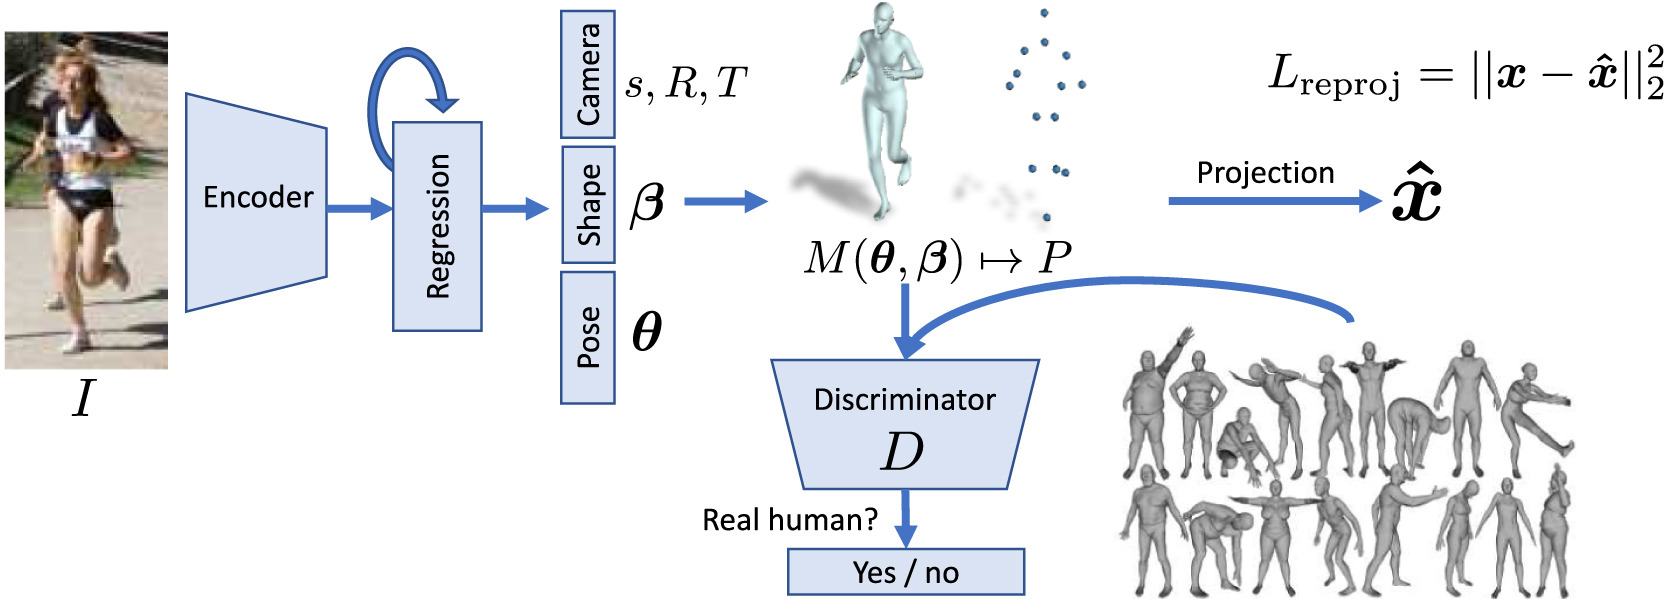
\includegraphics[scale=1.5]{images/chapter3/hmr_architecture.jpg}
	\caption[Αρχιτεκτονική του μοντέλου Human Mesh Recovery]{\textsl{Αρχιτεκτονική του μοντέλου Human Mesh Recovery}: H εικόνα περνάει από ένα συνελικτικό κωδικοποιητή, εξάγοντας τα χαρακτηριστικά της. Έπειτα, στέλνεται σε μία μονάδα επαναληπτικής παλινδρόμησης όπου γίνεται εκτίμηση της 3D αναπαράστασης του ανθρώπου, υπολογίζοντας τις παραμέτρους του μοντέλου SMPL. Η μονάδα παλινδρόμησης προσπαθεί να ελαχιστοποιήσει το σφάλμα της προβολής των σημείων κλειδιών. Οι εκτιμώμενες 3D παράμετροι περνάνε επίσης από έναν διαχωριστή D, στόχος του οποίου είναι να επαληθεύσει αν είναι πραγματικά εφικτή η πόζα.}
	\label{fig:hmr_architecture}
\end{figure}

 \begin{figure}[h]
	\centering
	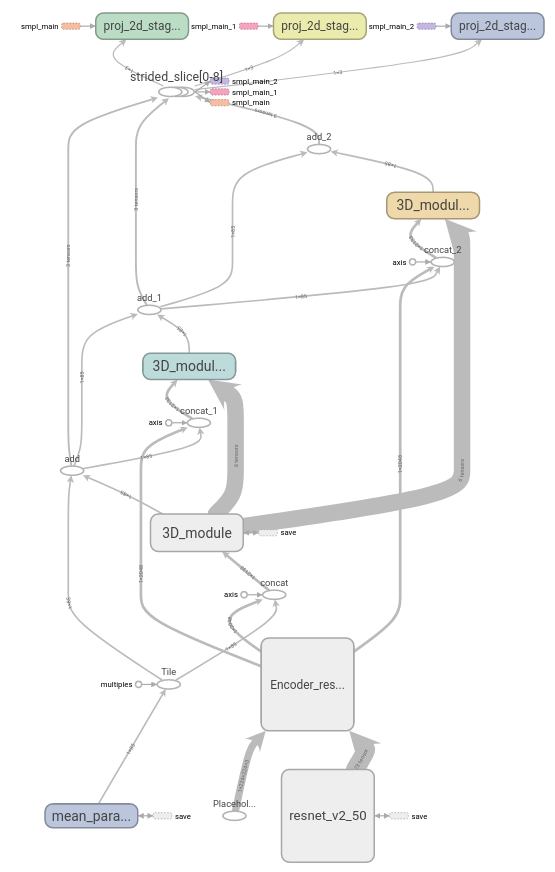
\includegraphics[scale=0.4]{images/chapter3/hmr_overall_architecture.png}
	\caption[Αρχιτεκτονική του δικτύου εκτίμησης Human Mesh Recovery - Tensorboard]{\textsl{Αρχιτεκτονική του δικτύου εκτίμησης του Human Mesh Recovery από το Tensorboard}: Τα χαρακτηριστικά της εικόνας εξάγονται από τον κωδικοποιητή \textsl{Encoder\_resnet}. Στην συνέχεια τα χαρακτηριστικά μαζί με τις τις παραμέτρους στέλνονται στον παλινδρομητή \textsl{3D\_module} 3 φορές. Στην πρώτη επανάληψη (\textsl{3\_module} γκρί) χρησιμοποιούνται οι μέσες τιμές των παραμέτρων, ενώ στις άλλες δύο (μπλε και κίτρινο) χρησιμοποιούνται οι εκτιμώμενοι παράμετροι από τη προηγούμενη επανάληψη. Οι παράμετροι στέλνονται στο μοντέλο SMPL, \textsl{smpl\_main}, παράγονται οι 3D κορυφές του πλέγματος και τα σημεία κλειδιά και μαζί με τις συντεταγμένες τις κάμερας στέλνονται στα τελικά 3 στάδια \textsl{proj\_2d\_stage}, όπου επιτελείται η προβολή των 3D σημείων κλειδιών σε 2D.}
	\label{fig:hmr_overall_architecture}
\end{figure}

Αναλυτικότερα, η είσοδος του νευρωνικού δικτύου για κάθε καρέ είναι μία εικόνα σμικρυσμένη σε διαστάσεις $224 \times 224$ πίξελ, διατηρώντας όμως την αρχική αναλογία διαστάσεων. Η επιλογή των μικρών διαστάσεων της εικόνας είναι απαραίτητη ώστε η εξαγωγή των χαρακτηριστικών της (και ολόκληρη η εκτίμηση πόζας) να γίνεται σε πραγματικό χρόνο.

Στη συνέχεια, η εξαγωγή των χαρακτηριστικών της εικόνας γίνεται από την μονάδα \textsl{Encoder\_resnet}, η οποία είναι το προ-εκπαιδευμένο μοντέλο του Tensorflow \href{https://github.com/tensorflow/models/blob/master/research/slim/nets/resnet\_v2.py}{resnet\_v2\_50} ταξινόμησης εικόνων πάνω στο σύνολο δεδομένων \href{https://www.image-net.org/}{ImageNet}. Με λίγα λόγια, το \textsl{resnet\_v2\_50} είναι ένα παραμένων συνελικτικό δίκτυο (residual convolutional network) αποτελούμενο από 4 μπλοκ με 50 συνολικά επίπεδα, όπως φαίνεται στο Σχήμα \ref{fig:resnet_block}. Αρχικά, υπάρχει ένα επίπεδο convolution\footnote{Η επεξήγηση των επιπέδων των νευρωνικών δικτύων γίνεται στο παράρτημα \ref{sec:nn_layers}.} και max-pooling με βήμα 2 και διαστάσεις πυρήνων $7 \times 7$ και $3 \times 3$ αντίστοιχα. Τα 4 μπλοκ αποτελούνται από 3, 4, 6 και 3 παραμένων μονάδες (residual units) αντίστοιχα των οποίων η δομή φαίνεται στο Σχήμα \ref{fig:residual_unit}. Τέλος, υπάρχουν ένα επίπεδο batch normalization, ένα επίπεδο ενεργοποίησης ReLU και ένα average pooling. \footnote{Αναφορικά, στο προ-εκπαιδευμένο δίκτυο resnet\_v2\_50 υπάρχει και ένα τελικό επίπεδο πλήρως συνδεδεμένο με 1000 κόμβους για την έξοδο κλάσης του ImageNet, το οποίο όμως δεν χρησιμοποιείται στην εκτίμηση πόζας.} Η έξοδος του \textsl{Encoder\_resnet} είναι τα χαρακτηριστικά της εικόνας $\phi \in \mathbb{R}^{2048}$.

\begin{figure}[h]
	\begin{subfigure}[h]{0.45\textwidth}
		\centering
		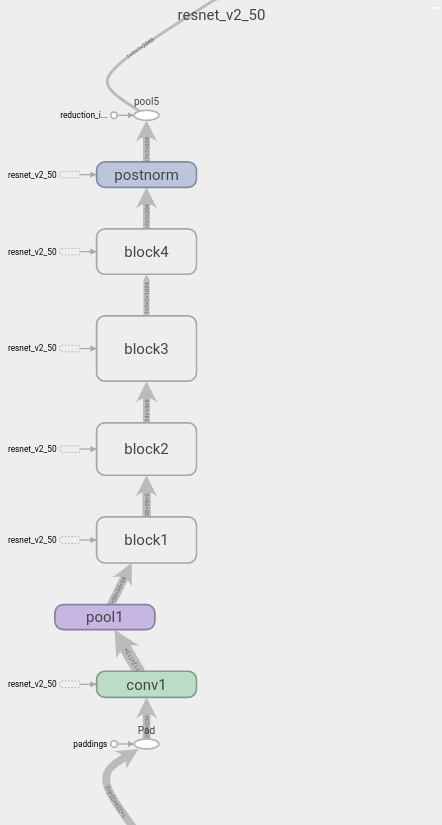
\includegraphics[width=\textwidth]{images/chapter3/resnet_v2_50.png}
	\end{subfigure} 
	\hfill
	\begin{subfigure}[h]{0.45\textwidth}
		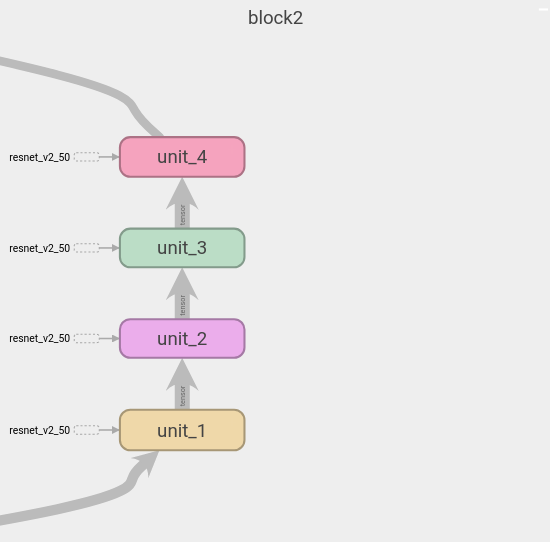
\includegraphics[width=\textwidth]{images/chapter3/resnet_block_example.png}
	\end{subfigure} 
	\caption[Tensorboard - Αρχιτεκτονική του resnet\_v2\_50]{Η αρχιτεκτονική του resnet\_v2\_50 όπως φαίνεται με χρήση του εργαλείου Tensorboard. Στα αριστερά φαίνονται τα 4 μπλοκς του resnet\_v2\_50 ενώ στα δεξιά φαίνονται τα 4 residual units του 2ου μπλοκ.}
	\label{fig:resnet_block}
\end{figure}

\begin{figure}[H]
	\centering
	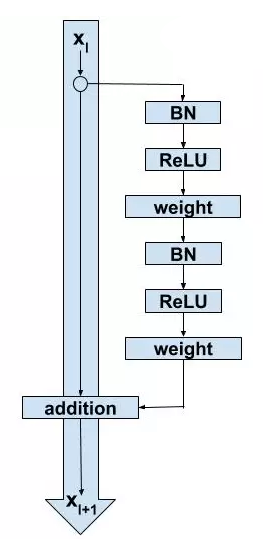
\includegraphics[scale=0.3]{images/chapter3/residual_block.png}
	\caption[Αρχιτεκτονική του residual unit του resnet\_v2\_50]{\textsl{Αρχιτεκτονική του residual unit του Resnet v2}: To κάθε residual unit αποτελείται από τα εξής επίπεδα Batch Normalization, ReLU, Convolution, Batch Normalization και Convolution. Επιπλέον, υπάρχει και μία ταυτοτική σύνδεση με το επόμενο residual unit, δίνοντας την δυνατότητα να παραλειφθούν τα αναφερόμενα επίπεδα.}
	\label{fig:residual_unit}
\end{figure} 

To δίκτυο ResNet χρησιμοποιεί κατά κόρων επίπεδα Batch Normalization, ρυθμίζοντας την μέση τιμή και διακύμανση των δεδομένων εισόδου σε κάθε επίπεδο και βελτιώνοντας έτσι την απόδοση του δικτύου. Τοιουτοτρόπως, εξαλείφεται το πρόβλημα της μεταβολής των στατιστικών χαρακτηριστικών μεταξύ των δεδομένων εκπαίδευσης και του πραγματικού κόσμου. Στην εφαρμογή της εκτίμησης πόζας, το γεγονός αυτό είναι άκρως σημαντικό καθώς η αβεβαιότητα των συνθηκών περιβάλλοντος, του φωτισμού ή και της ενδυμασίας του χρήστη είναι δεδομένα.

Ένα άλλο χαρακτηριστικό του ResNet είναι η χρήση των ταυτοτικών συνδέσεων μεταξύ των residual units. Από την μία πλευρά, αυτό επιτρέπει στο δίκτυο να μάθει μία ταυτοτική συνάρτηση εξασφαλίζοντας ότι το υψηλότερα επίπεδα θα έχουν τουλάχιστον τόσο καλή απόδοση όσο τα χαμηλότερα επίπεδα και σίγουρα όχι χειρότερη. Από την άλλη πλευρά και ίσως η πιο σημαντική, είναι ότι επιτρέπουν στο ανάδελτα του σφάλματος να ρεύσει προς τα αρχικά επίπεδα μέσω αυτού του εναλλακτικού μονοπατιού. Με αυτόν τον τρόπο, αντιμετωπίζεται το πρόβλημα του εξαφανιζόμενου ανάδελτα σφάλματος (vanishing gradient problem) καθιστώντας την εκπαίδευση βαθιών νευρικών δικτύων δυνατή \cite{identity_mappings}.

Στο Σχήμα \ref{fig:3d_module} φαίνεται η μονάδα 3D παλινδρόμησης, η οποία αποτελείται από 2 πλήρως συνδεδεμένα επίπεδα με 1024 κόμβους το καθένα και ένα επίπεδο dropout μεταξύ τους, ακολουθούμενα από ένα τελικό πλήρως συνδεδεμένο επίπεδο με 85 κόμβους. Η έξοδος του 3D\_module λοιπόν είναι το διάνυσμα $\Theta \in \mathbb{R}^{85}$, το οποίο αποτελείται αναλυτικά από 

\begin{itemize}
	\item τις παραμέτρους πόζας $\theta \in \mathbb{R}^{72}$, που είναι οι περιστροφές ανά άξονα, δηλαδή οι 3 γωνίες των 24 αρθρώσεων.
	\item τις παραμέτρους σχήματος $\beta \in \mathbb{R}^{10}$, που καθορίζουν την μορφή του ανθρώπινου σώματος, δηλαδή το ύψος, βάρος και αναλογία οστών.
	\item τις 3D συντεταγμένες θέσεως της κάμερας.
\end{itemize}

\begin{figure}[H]
	\centering
	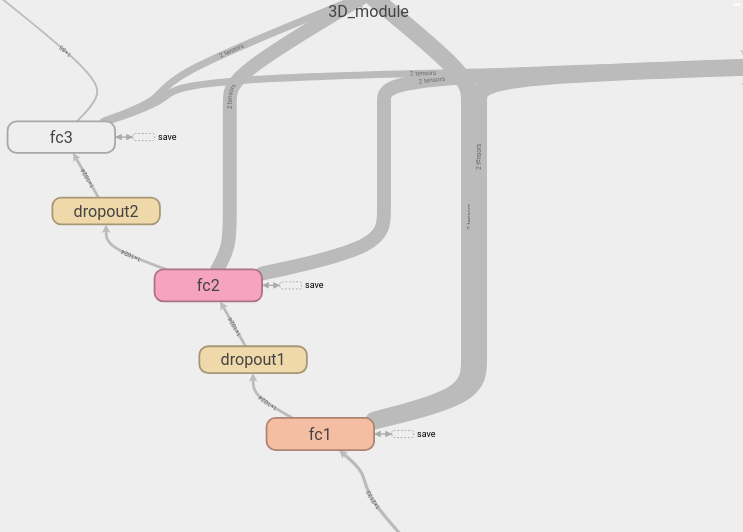
\includegraphics[scale=0.5]{images/chapter3/3d_module.png}
	\caption{Tensorboard - Αρχιτεκτονική της μονάδας 3D\_module}
	\label{fig:3d_module}
\end{figure}

Όπως έχει αναφερθεί, η τελική έξοδος της εκτίμησης πόζας προκύπτει από την εκτέλεση 3 φορών της μονάδας 3D\_module, όπου η είσοδος κάθε φορά είναι οι παράμετροι $\Theta$ της προηγούμενης επανάληψης και τα χαρακτηριστικά της εικόνας $\phi$.